\documentclass[greek]{beamer}
%\usepackage{fontspec}
\usepackage{amsmath,amsthm}
\usepackage{unicode-math}
\usepackage{xltxtra}
\usepackage{graphicx}
\usetheme{CambridgeUS}
\usecolortheme{seagull}
\usepackage{hyperref}
\usepackage{ulem}
\usepackage{xgreek}

\usepackage{pgfpages}
\usepackage{tikz}
\usepackage{tkz-tab}
%\setbeameroption{show notes on second screen}
%\setbeameroption{show only notes}

\setsansfont{Noto Serif}

\usepackage{multicol}

\usepackage{appendixnumberbeamer}

\setbeamercovered{transparent}
\beamertemplatenavigationsymbolsempty

\title{Συναρτήσεις}
\subtitle{Συνέπειες Bolzano 2 (the rest)}
\author[Λόλας]{Κωνσταντίνος Λόλας}
\date{}

\begin{document}

\begin{frame}
 \titlepage
\end{frame}

\section{Θεωρία}
\begin{frame}{Ένα μάθημα μόνο θεωρία}
 \begin{itemize}
  \item<1-> Φτιάξτε άξονες
  \item<2-> Σχεδιάστε συνεχή συνάρτηση στο διάστημα $[0,1]$ που δεν έχει μέγιστο ή ελάχιστο
 \end{itemize}
 \onslide<3>Συμπέρασμα...
\end{frame}

\begin{frame}{Θεώρημα 1}
 \begin{block}{Θεώρημα μέγιστου ελάχιστου}
  Κάθε συνεχής σε κλειστό διάστημα συνάρτηση $f$ έχει μέγιστο ΚΑΙ ελάχιστο στο $Δ$.
 \end{block}
\end{frame}

\begin{frame}{Δοκιμασία}
 \begin{itemize}
  \item<1-> Φτιάξτε άξονες
  \item<2-> Σχεδιάστε συνεχή συνάρτηση στο διάστημα $[0,1]$ με σύνολο τιμών το $[2,3]$
  \item<3-> Δοκιμάστε να δημιουργήσετε άλλη συνάρτηση που να μην περνάει τώρα από το $2.5$
 \end{itemize}
 \onslide<4>Συμπέρασμα...
\end{frame}

\begin{frame}{Θεώρημα 2}
 \begin{block}{Θεώρημα ενδιαμέσων τιμών (γενίκευση Bolzano)}
  Έστω μια συνεχής συνάρτηση $f$ στο $[α,β]$ με $f(α)=κ$ και $f(β)=λ$ με $λ\ne κ$. Για κάθε $η\in (κ,λ)$ υπάρχει $x_0\in (α,β)$ ώστε $f(x_0)=η$
 \end{block}
\end{frame}

\begin{frame}{Θεώρημα 3}
 \begin{block}{Θεώρημα εικόνας διαστήματος συνεχούς συνάρτησης}
  Έστω μια συνεχής συνάρτηση $f$ στο $[α,β]$. Η εικόνα $f([α,β])$ είναι και πάλι διάστημα.
 \end{block}
\end{frame}

\begin{frame}{Φαντασία με Σ-Λ}
 \begin{itemize}
  \item<1-> Γνησίως αύξουσα σε διάστημα έχει πάντα μέγιστο
  \item<2-> Γνησίως αύξουσα σε κλειστό διάστημα έχει πάντα μέγιστο  Πού?
 \end{itemize}
 \onslide<3->Συμπέρασμα...
\end{frame}

\begin{frame}{Θεώρημα 4}
 \begin{block}{Θεώρημα συνεχών γνησίως μονότονων συναρτήσεων σε διάστημα}
  Έστω μια συνεχής στο $[α,β]$, γνησίως αύξουσα συνάρτηση $f$.
  \begin{itemize}
   \item<1-> $f([α,β])=[f(α),f(β)]$
   \item<2-> $f([α,β))=[f(α),\lim\limits_{x \to β^-}{ f(x) })$
   \item<3-> $f((α,β])=(\lim\limits_{x \to α^+}{ f(x) },f(β)]$
   \item<4-> $f((α,β))=(\lim\limits_{x \to α^+}{ f(x) },\lim\limits_{x \to β^-}{ f(x) })$
  \end{itemize}
 \end{block}
 \onslide<5>Με λίγα λόγια

 Ή φτάνουμε την τιμή Ή πλησιάζουμε συνεχώς
\end{frame}

\section{Ασκήσεις}
\subsection{Άσκηση 1}
\begin{frame}[label=Άσκηση1]{Εξάσκηση 1}
 Δίνεται η συνάρτηση $f(x)=2^x$. Να δείξετε ότι υπάρχει $ξ\in (10,11)$ ώστε $f(ξ)=2023$.

 \hyperlink{Λύση1}{\beamerbutton{Λύση}}
\end{frame}

\subsection{Άσκηση 2}
\begin{frame}[label=Άσκηση2]{Εξάσκηση 2}
 Έστω η συνεχής και γνησίως φθίνουσα συνάρτηση $f:[1,3]\to\mathbb{R}$. Να δείξετε ότι υπάρχει ακριβώς ένα $x_0\in (1,3)$ ώστε
 $$f(x_0)=\frac{f(1)+f(2)+f(3)}{3}$$

 \hyperlink{Λύση2}{\beamerbutton{Λύση}}
\end{frame}

\subsection{Άσκηση 3}
\begin{frame}[label=Άσκηση3]{Εξάσκηση 3}
 Δίνεται η συνάρτηση $f(x)=(x-1)^4(x-3)^2$, $x\in \mathbb{R}$. Να αποδείξετε ότι η $f$ έχει δύο θέσεις ελαχίστων $x_1$, $x_2$ με $x_1<x_2$. Στη συνέχεια να δείξετε ότι υπάρχει ένα τουλάχιστον $x_0\in (x_1,x_2)$ που η συνάρτηση παρουσιάζει μέγιστο στο $[x_1,x_2]$.

 \hyperlink{Λύση3}{\beamerbutton{Λύση}}
\end{frame}

\subsection{Άσκηση 4}
\begin{frame}[label=Άσκηση4]{Εξάσκηση 4}
 Έστω $f:[1,2]\to\mathbb{R}$ μία συνεχής συνάρτηση της οποίας η γραφική παράσταση βρίσκεται πάνω από την ευθεία $ε:y=x$. Να δείξετε ότι υπάρχει ένα τουλάχιστον σημείο της $C_f$ που απέχει από την ευθεία $ε$ περισσότερο από ότι απέχουν τα υπόλοιπα σημεία της $C_f$.

 \hyperlink{Λύση4}{\beamerbutton{Λύση}}
\end{frame}

\subsection{Άσκηση 5}
\begin{frame}[label=Άσκηση5]{Εξάσκηση 5}
 Έστω η συνεχής συνάρτηση $f:[2,4]\to\mathbb{R}$. Να δείξετε ότι υπάρχει ενα τουλάχιστον $x_0\in (2,4)$ ώστε
 $$f(x_0)=\frac{f(2)+2f(3)+3f(4)}{6}$$

 \hyperlink{Λύση5}{\beamerbutton{Λύση}}
\end{frame}

\subsection{Άσκηση 6}
\begin{frame}[label=Άσκηση6]{Εξάσκηση 6}
 Δίνεται η συνάρτηση $f(x)=e^x+x$
 \begin{itemize}
  \item<1-> Να βρείτε το σύνολο τιμών της $f$
  \item<2-> Να βρείτε το $f(Β)$ όταν
        \begin{itemize}
         \item<3-> $Β=[0,1]$
         \item<4-> $Β=[0,1)$
         \item<5-> $Β=(-\infty,0]$
        \end{itemize}
  \item<6-> Να βρείτε τη μέγιστη και την ελάχιστη τιμή της $f$, όταν είναι ορισμένη στο $Β=[0,1]$.
 \end{itemize}

 \hyperlink{Λύση6}{\beamerbutton{Λύση}}
\end{frame}

\subsection{Άσκηση 7}
\begin{frame}{Εξάσκηση 7}
 Δίνεται η συνάρτηση $f(x)=\frac{1}{x}-\ln x$
 \begin{enumerate}
  \item<1-> Να δείξετε ότι η $f$ αντιστρέφεται και να βρείτε το πεδίο ορισμού της $f^{-1}$
  \item<2-> Να δείξετε ότι η εξίσωση $f(x)=2023$ έχει ακριβώς μία ρίζα
  \item<3-> Να εξετάσετε αν υπάρχει $x_0\in (0,1]$ τέτοιο ώστε $f(x_0)=e^{x_0}-2$
 \end{enumerate}
\end{frame}

\subsection{Άσκηση 8}
\begin{frame}{Εξάσκηση 8}
 Έστω $f:\mathbb{R}\to\mathbb{R}$ μία συνεχής συνάρτηση. Στο σχήμα φαίνονται τα διαστήματα μονοτονίας της $f$ και οι οριακές τιμές της στο $-\infty$ και στο $+\infty$.

 \centering
 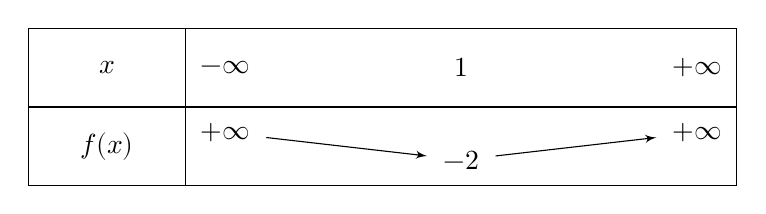
\begin{tikzpicture}
  \tkzTabInit  {$x$ / 1 , $f(x)$ / 1 }
  {$-\infty$, $1$, $+\infty$}
  \tkzTabVar{+/ $+\infty$, -/$-2$/, +/ $+\infty$ / }
 \end{tikzpicture}
 \begin{itemize}
  \item<1-> Να βρείτε το σύνολο τιμών της $f$
  \item<2-> Να δείξετε ότι η συνάρτηση έχει ακριβώς δύο ρίζες
  \item<3-> Να βρείτε το πλήθος των ριζών της εξίσωσης $f(x)=α$ για τις διάφορες τιμές του $α\in\mathbb{R}$
 \end{itemize}
\end{frame}

\subsection{Άσκηση 9}
\begin{frame}{Εξάσκηση 9}
 Δίνεται η συνάρτηση $f(x)=\begin{cases}
   e^x+x,       & x\le 0 \\
   1-\ln (x+1), & x>0
  \end{cases}$
 \begin{enumerate}
  \item<1-> Να δείξετε ότι η $f$ είναι συνεχής και να βρείτε το σύνολο τιμών της
  \item<2-> Να δείξετε ότι η η $f$ έχει ακριβώς δύο ρίζες ετερόσημες
  \item<3-> Αν $x_1$, $x_2$ $(x_1<x_2)$ οι ρίζες του ερωτήματος 2., να δείξετε ότι η εξίσωση
        $$\frac{f(α)-1}{x-x_1}+\frac{f(β)-1}{x-x_2}=0$$
        έχει τουλάχιστον μία ρίζα στο διάστημα $(x_1,x_2)$ για κάθε $α$, $β\in\mathbb{R}-{0}$
  \item<4-> Αν $κ\le 0\le λ$ και ισχύει $e^κ-1=\ln (λ+1)-κ$, να βρείτε τις τιμές $κ$ και $λ$.
 \end{enumerate}
\end{frame}

\subsection{Άσκηση 10}
\begin{frame}{Εξάσκηση 10}
 Έστω $f:\mathbb{R}\to\mathbb{R}$ μία συνάρτηση η οποία είναι συνεχής, γνησίως φθίνουσα και έχει σύνολο τιμών το $f(\mathbb{R})=(0,+\infty)$. Να βρείτε τα όρια:
 \begin{enumerate}
  \item<1-> $\lim\limits_{x \to +\infty}{ \frac{f(x)-x}{x+f(x)} }$
  \item<2-> $\lim\limits_{x \to -\infty}{ \frac{e^x}{f(x)} }$
  \item<3-> $\lim\limits_{x \to +\infty}{ \frac{\ln f(x)}{f(x)} }$
 \end{enumerate}
\end{frame}

\subsection{Άσκηση 11}
\begin{frame}{Εξάσκηση 11}
 Έστω $f:Α\to\mathbb{R}$ μία συνάρτηση με $Α=(0,+\infty)$ με $f(x)=\frac{1}{x}-x+1$.
 \begin{enumerate}
  \item<1-> Να βρείτε το σύνολο τιμών της
  \item<2-> Να δείξετε ότι υπάρχει η αντίστροφη συνάρτηση $f^{-1}$ και ότι είναι γνησίως φθίνουσα
  \item<3-> Αν θεωρήσουμε γνωστό ότι η $f^{-1}$ είναι συνεχής, να βρείτε τα όρια:
        \begin{itemize}
         \item $\lim\limits_{x \to +\infty}{ \frac{1}{f^{-1}(x)} }$
         \item<4-> $\lim\limits_{x \to +\infty}{ \frac{f^{-1}(x)-x}{x+f^{-1}(x)} }$
         \item<5-> $\lim\limits_{x \to -\infty}{ \frac{1}{f^{-1}(x)} }$
        \end{itemize}
 \end{enumerate}
\end{frame}

\subsection{Άσκηση 12}
\begin{frame}{Εξάσκηση 12}
 Έστω $f:[0,1]\to\mathbb{R}$ μία συνάρτηση η οποία είναι $1-1$, συνεχής και ισχύει
 $$0<f(0)<1$$
 Να δείξετε ότι $f(x)\ne 0$ για κάθε $x\in [0,1]$
\end{frame}

\subsection{Άσκηση 13}
\begin{frame}{Εξάσκηση 13}
 Να βρείτε όλες τις συνεχείς συναρτήσεις $f:\mathbb{R}\to\mathbb{R}$, για τις οποίες ισχύει $f^3(x)=f(x)$ για κάθε $x\in\mathbb{R}$
\end{frame}

\section{}
\begin{frame}
 Στο moodle θα βρείτε τις ασκήσεις που πρέπει να κάνετε, όπως και αυτή τη παρουσίαση
\end{frame}

\appendix
\section{Λύσεις Ασκήσεων}
\begin{frame}
 \tableofcontents
\end{frame}

\subsection{Άσκηση 1}
\begin{frame}[label=Λύση1]
 Με θεώρημα ενδιαμέσων τιμών. Η συνάρτηση είναι συνεχής στο $[10,11]$ με $f(10)=1024$ και $f(11)=2048$. Αφού $2023\in (1024,2048)$ υπάρχει $x_0$...

 \hyperlink{Άσκηση1}{\beamerbutton{Πίσω στην άσκηση}}
\end{frame}

\subsection{Άσκηση 2}
\begin{frame}[label=Λύση2]
 Με Bolzano ή με μέγιστης ελάχιστης τιμής και ΘΕΤ.

 \begin{gather*}
  f(3)<f(2)<f(1) \\
  3f(3)<f(1)+f(2)+f(3)<3f(1) \\
  f(3)<\frac{f(1)+f(2)+f(3)}{3}<f(1)
 \end{gather*}

 \hyperlink{Άσκηση2}{\beamerbutton{Πίσω στην άσκηση}}
\end{frame}

\subsection{Άσκηση 3}
\begin{frame}[label=Λύση3]
 Προφανές ελάχιστο στα $x_1=1$ και $x_2=3$. Ως συνεχής στο $[1,3]$ έχει σίγουρα ΚΑΙ μέγιστο στο $(1,3)$

 \hyperlink{Άσκηση3}{\beamerbutton{Πίσω στην άσκηση}}
\end{frame}

\subsection{Άσκηση 4}
\begin{frame}[label=Λύση4]
 Η συνάρτηση `απόστασης` $f(x)-x$ είναι ορισμένη στο κλειστό διάστημα και έχει σίγουρα μέγιστο

 \hyperlink{Άσκηση4}{\beamerbutton{Πίσω στην άσκηση}}
\end{frame}

\subsection{Άσκηση 5}
\begin{frame}[label=Λύση5]
 Όμοια με την Άσκηση 2

 \hyperlink{Άσκηση5}{\beamerbutton{Πίσω στην άσκηση}}
\end{frame}

\subsection{Άσκηση 6}
\begin{frame}[label=Λύση6]
 \begin{enumerate}
  \item Είναι γνησίως αύξουσα άρα $(f(+\infty),f(-\infty))$
  \item Προφανώς $[f(0),f(1)]$...
 \end{enumerate}

 \hyperlink{Άσκηση6}{\beamerbutton{Πίσω στην άσκηση}}
\end{frame}

\end{document}
